% !TEX root = ../thesis.tex
\chapter{Movish recommendation system for movies}
\label{chapter:<movish_system>}

\subsection{Introduction}
\label{sec:movish_introduction}

In this chapter the reader can understand the basic architecture of Movish. Since implementing a recommendation system is a challenging process we will explain how all the problems encountered have been addressed either by design or by system architecture. This chapter is thus fundamental to all the readers that want to understand the basic functions and architecture of the system.
We will start from the basic system that inspired Movish: ContentWise and Milo, and then we will analyze Movish itself.

\subsection{ContentWise}
\label{sec:contentwise}

ContentWise is a well known recommendation system developer by the \ac{DEI} of Politecnico di Milano university. This product basically exposed a movie catalog and makes the use able to perform ratings and obtain recommendations using different algorithms. The user is able to change the recommendation system by itself and the interface is designed to be used by recommendation system professionals. The figure \ref{fig:contentwise} shows ContentWise home page.    

\begin{figure}
  \centering
  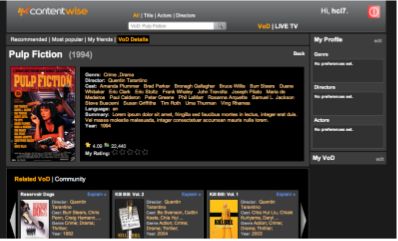
\includegraphics[width=0.9\textwidth]{figures/contentwise-homepage.png}
  \caption{ContentWise}
  \label{fig:contentwise}
\end{figure}

From a first look it is clear that the \ac{GUI} has a late 90' style. The architecture of ContentWise is also very rigid: the algorithms are embedded in the \ac{GUI} and this makes the action of adding a new algorithm really troublesome.
The application is mainly written in Java programming language.
The inability of adding a new algorithm easily and the overcomplicated user interface of ContentWise made the system not suitable for a system that is able to research on new algorithms on unaware users.

\subsection{Milo}
\label{sec:milo}

During the 2011/2012 course of digital and internet television a new recommendation system for movies that wanted to be similar to ContentWise but more modular and flexible such that it was easy to add new algorithms was implemented.
Since there wanted to be clear distinction between the engine and the presentation a \ac{MVC} \cite{mvc} paradigm has been used. Due to the python programming language popularity and emerging web frameworks, it has been chosen as base language. Among all the available frameworks, Pyramid \cite{pyramid} has been selected thanks to its flexibility and easy to use.
In fact Pyramid allows to have a base \ac{MVC} framework skeleton and plug it with all the libraries you need for your application. Also modifying the base components it is easy and suggested by developers to fully satisfy the application needs. In particular Milo had to communicate with a matlab \cite{matlab} based set of algorithms. Thanks to pymatlab \cite{pymatlab}, python is able to talk directly to matlab in a way that reminds a server-client socket communication.
As stated in chapter \ref{chapter:<Overview>}, recommendation systems perform recommendations using a model. This model requires a lot of computational power and time. Web applications have a better user experience if they have a lower page load delay instead. To overcome this conflicting needs a asynchronous task manager framework has been integrated to allow the web application to trigger some events that add new tasks. These tasks are thus run on a separate process.
In order to make the administrator able to add unmodified Matlab \cite{matlab} algorithms the pymatlab \cite{pymatlab} library has been used. Pymatlab makes python be able to communicate with matlab via the matlab shell using accessible via a socket like interface. Figure \ref{fig:urm_creation_code} shows a piece of code of the creation of the \ac{URM} from the python side.

\begin{figure}
  \centering
  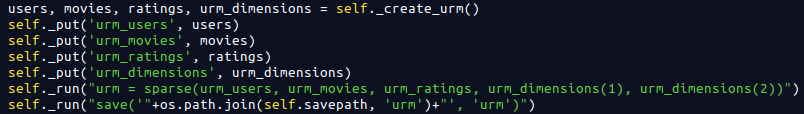
\includegraphics[width=\textwidth]{figures/urm_creation_code.png}
  \caption{URM creation code}
  \label{fig:urm_creation_code}
\end{figure}

The ``self.create_urm()'' generates the urm picking the data from the database. That python function returns a numpy array of users, movies, rating e and array indicating the dimension of the the matrix. The dimension is needed to create a sparse matrix of the right size. In fact the ``self.create_urm()'' function only returns actual data, skipping all the zeros. This avoid not necessary usage of ram due to too big matrices. Line from 2 to 5 put the variables in the matlab environment. Line 6 creates the sparse matrix into the matlab environment. The matrix created so is then stored as a .mat file for later use during the creation of the model.
As you can see all the communication is handled by running string like commands. Variables are stored and retrieved from the matlab environment thanks to the ``get'' and ``put'' functions of Figure \ref{fig:matlab_put_get_code}.

\begin{figure}
  \centering
  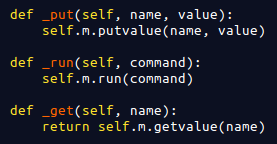
\includegraphics[width=0.4\textwidth]{figures/matlab_put_get_code.png}
  \caption{Code for the python\-matlab communication}
  \label{fig:matlab_put_get_code}
\end{figure}

This allows a clean separation of the python environment and the matlab environment. All the variables are transferred as strings or as floats. This is a limitation of the pymatlab library which is not able to handle integers variable correctly. Also all variables from python to matlab must be numpy \cite{numpy} arrays.

NumPy is the fundamental package for scientific computing with Python. It contains useful function and data structures for easy management of matrices and numerical data arrays. Together with scipy \cite{scipy}, numpy wants to be an open source alternative to matlab providing software for mathematics, science and engineering. Scipy is built on top of numpy.

Milo was developed in a modular way and was the union of two subsystems \cite{thesis-andreia}: a graphical engine and a recommendation engine called Whisperer. Whisperer was in charge of communicating with matlab through the just exposed pymatlab interface. The graphical engine was able to communicate with Whisperer thanks to a rest interface. In order to clarify reader understanding of Milo architecture the user can refer to Figure \ref{fig:milo_architecture}.

\begin{figure}
  \centering
  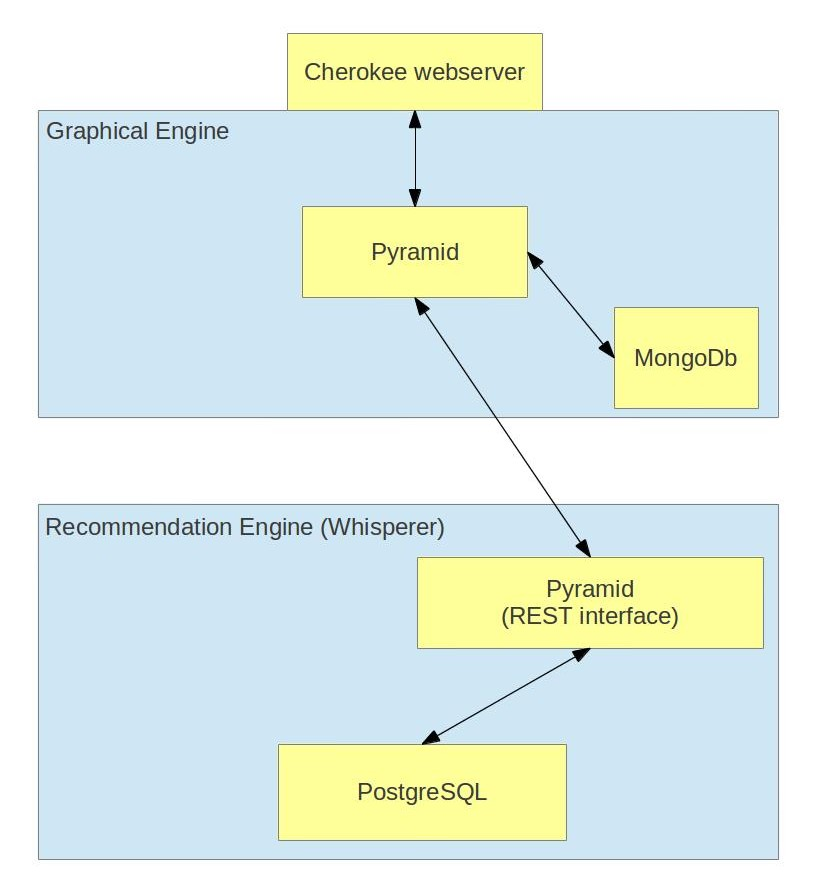
\includegraphics[width=0.7\textwidth]{figures/milo_architecture.jpg}
  \caption{Milo architecture}
  \label{fig:milo_architecture}
\end{figure}

CONTINUE HERE EXPLANING THE FIGURE


In Figure \ref{fig:movish_homepage} the reader can see the movish.co homepage. 

\begin{figure}
  \centering
  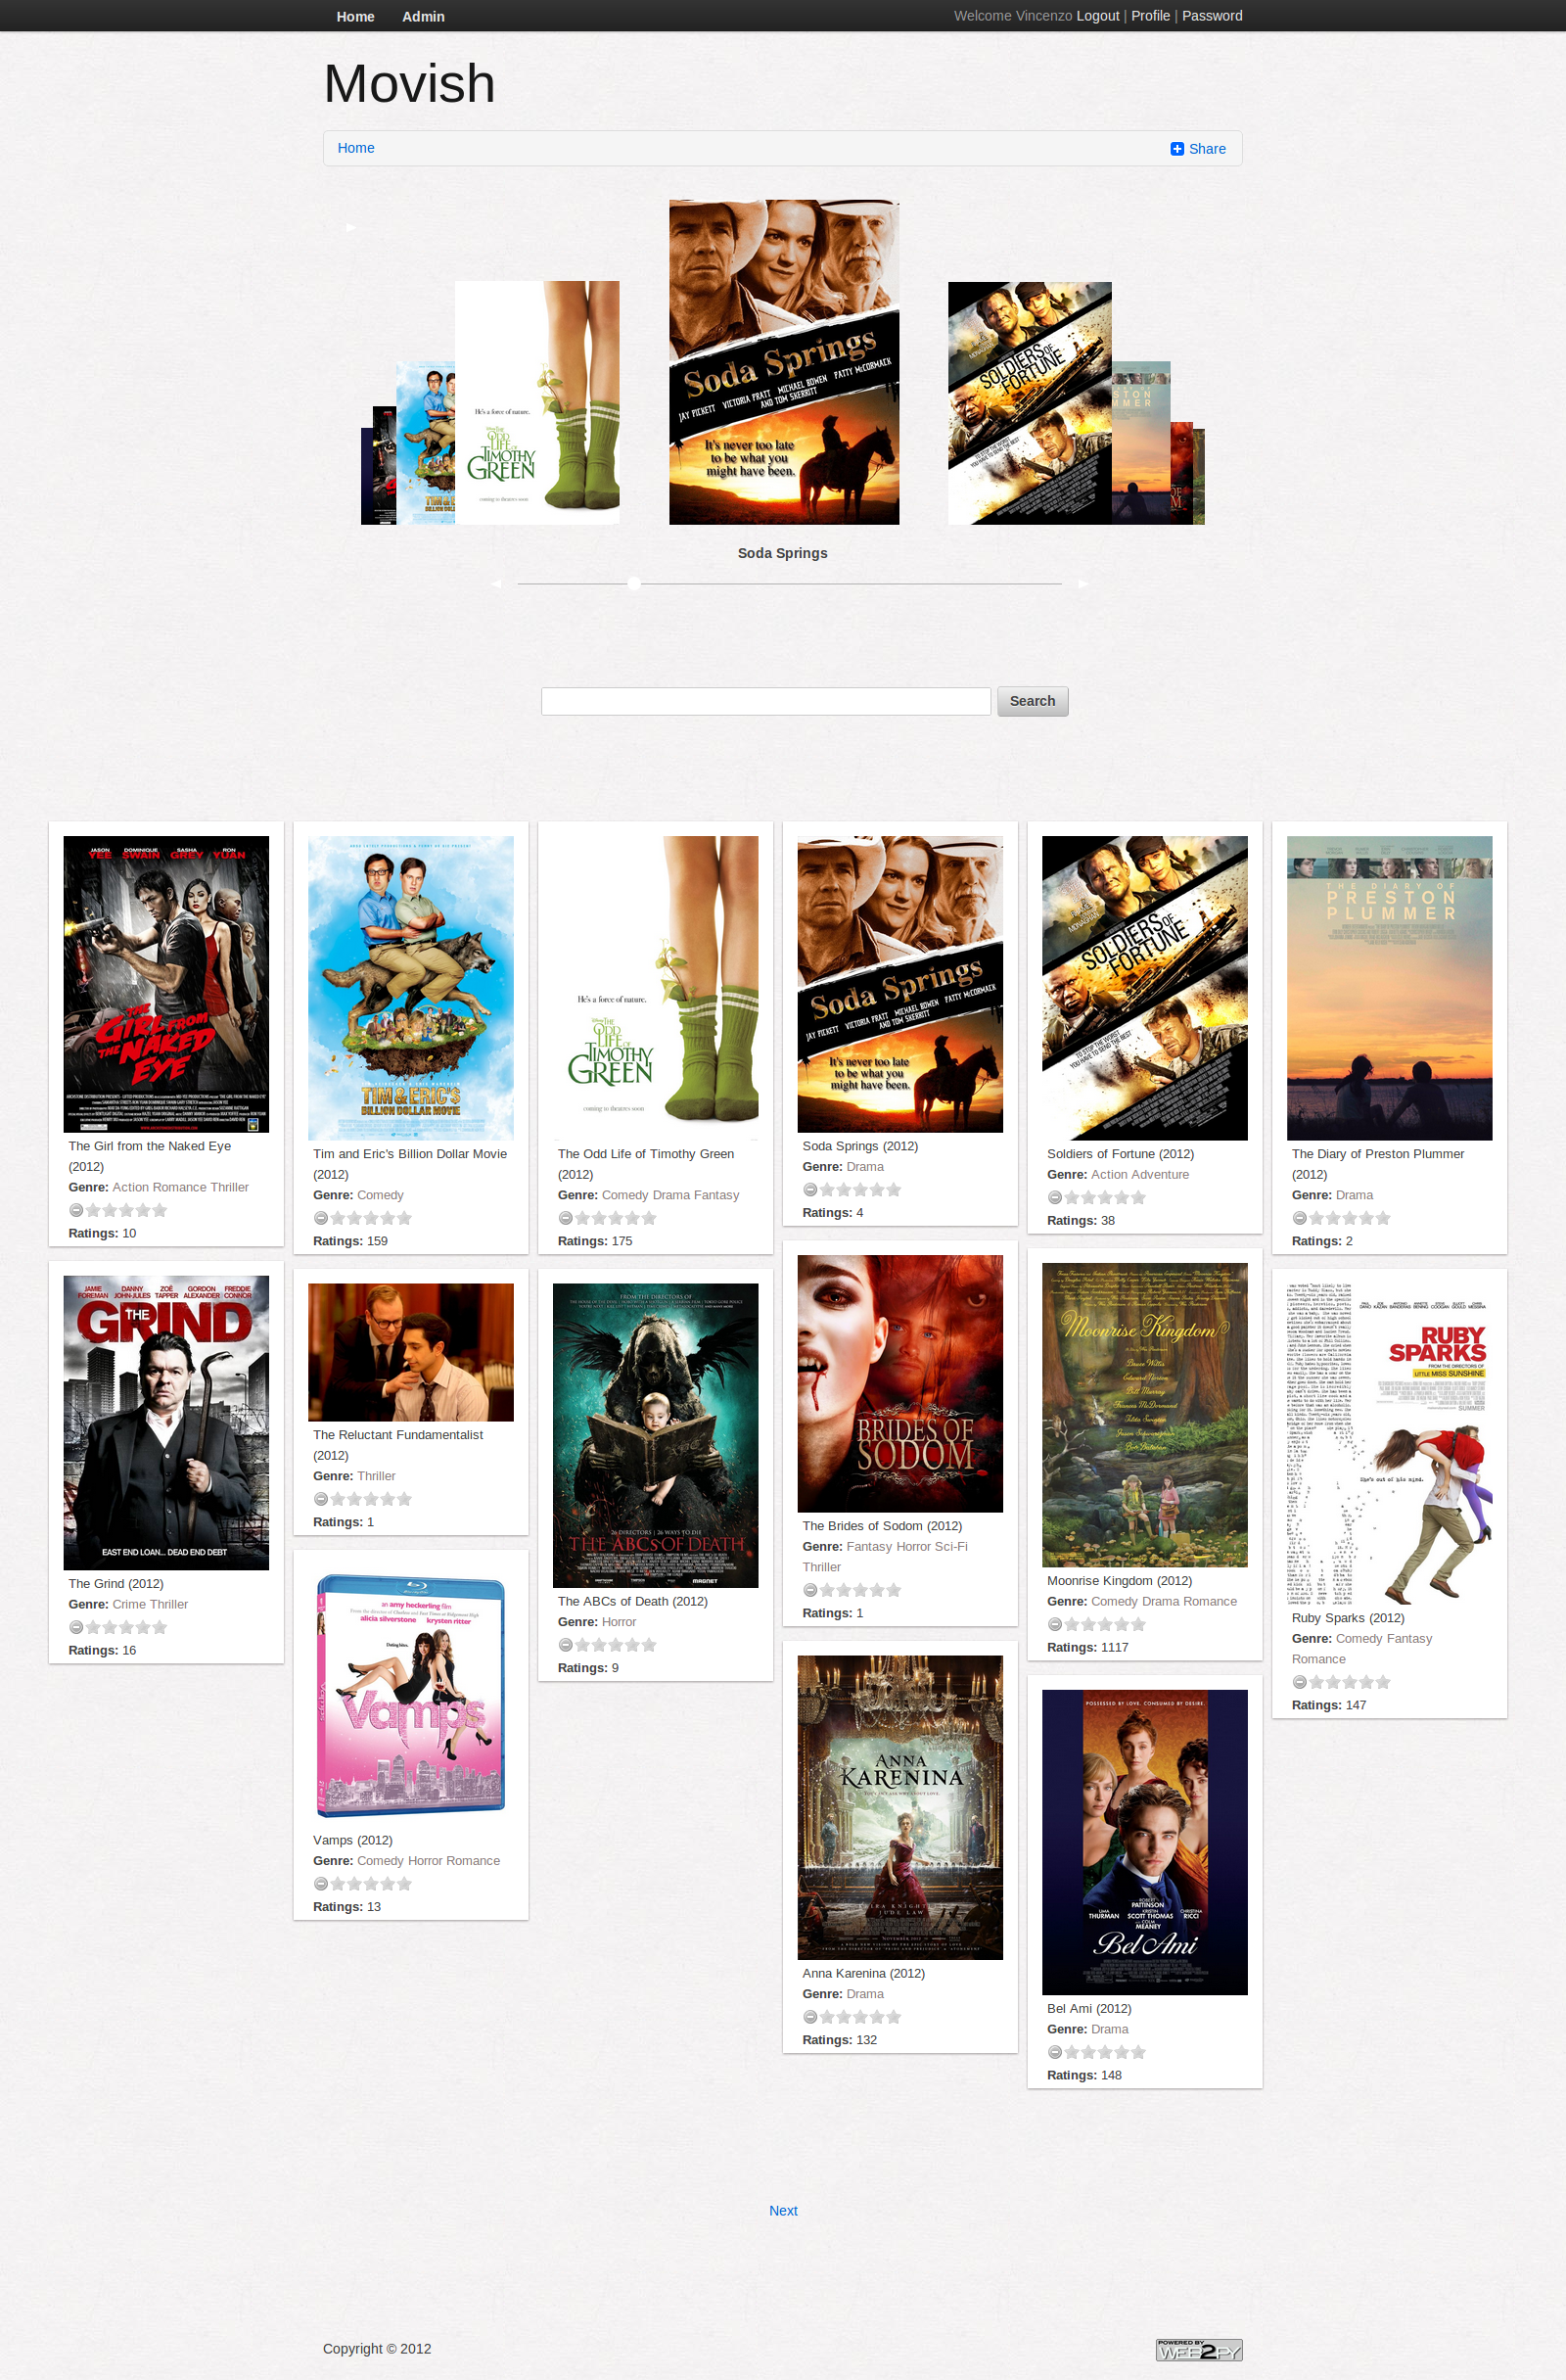
\includegraphics[width=0.7\textwidth]{figures/movish-homepage.png}
  \caption{Movish homepage}
  \label{fig:movish_homepage}
\end{figure}


\acresetall